\section{Comparison to GLIDE and DALL-E 2}
\label{sec:benchmark_comparison}

\cref{fig:drawit_vs_dalle2_detailed_alignment} shows category wise comparison between \name and DALL-E 2 \cite{ramesh-dalle2} on \benchmarkname. We observe that human raters clearly prefer \name over DALL-E 2 in 7 out of 11 categories for text alignment. For sample fidelity, they prefer \name over DALL-E 2 in all 11 categories. \Cref{fig:drawit_vs_dalle2_reddit,fig:drawit_vs_dalle2_colors,fig:drawit_vs_dalle2_conflicting,fig:drawit_vs_dalle2_dalle,fig:drawit_vs_dalle2_text} show few qualitative comparisons between \name and DALL-E 2 samples used for this human evaluation study. Some of the categories where \name has a considerably larger preference over DALL-E 2 include Colors, Positional, Text, DALL-E and Descriptions. The authors in \cite{ramesh-dalle2} identify some of these limitations of DALL-E~2, specifically they observe that DALLE-E~2 is worse than GLIDE \cite{nichol-glide} in binding attributes to objects such as colors, and producing coherent text from the input prompt (cf.\ the discussion of limitations in \cite{ramesh-dalle2}). To this end, we also perform quantitative and qualitative comparison with GLIDE \cite{nichol-glide} on \benchmarkname. See \cref{fig:drawit_vs_glide_detailed_alignment} for category wise human evaluation comparison between \name and GLIDE. See \Cref{fig:drawit_vs_glide_reddit,fig:drawit_vs_glide_colors,fig:drawit_vs_glide_conflicting,fig:drawit_vs_glide_dalle,fig:drawit_vs_glide_text} for qualitative comparisons. \name outperforms GLIDE on 8 out of 11 categories on image-text alignment, and 10 out of 11 categories on image fidelity. We observe that GLIDE is considerably better than DALL-E~2 in binding attributes to objects corroborating the observation by  \citep{ramesh-dalle2}.


\begin{figure}
    \centering
    \begin{subfigure}[t]{\textwidth}
    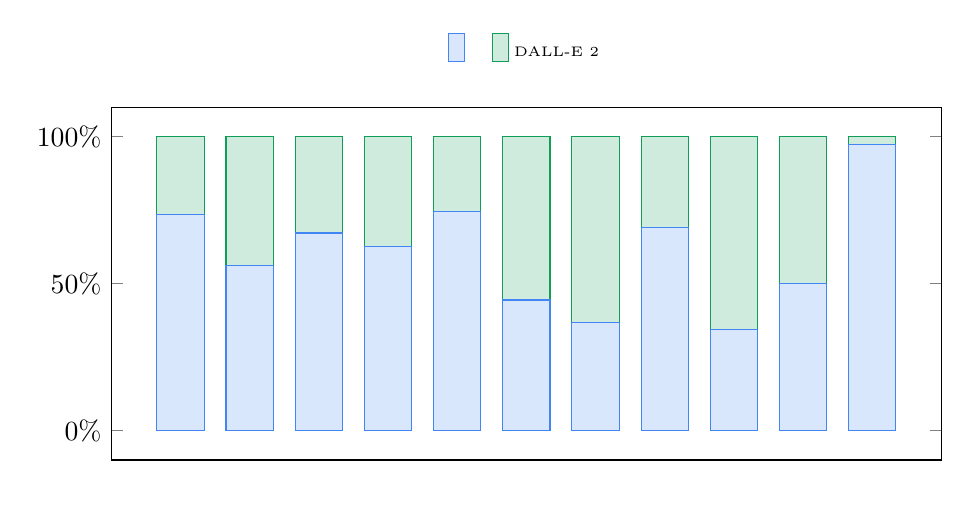
\begin{tikzpicture}

\definecolor{google_blue}{RGB}{66,133,244}
\definecolor{google_red}{RGB}{219,68,55}
\definecolor{google_yellow}{RGB}{194,144,0}
\definecolor{google_green}{RGB}{15,157,88}

\begin{axis}[
name=fidelity,
width=\textwidth,
height=0.5\textwidth,
ybar stacked,
ymin=-0.1,
ymax=1.1,
xtick=data,
xtick style={draw=none},
symbolic x coords={Colors,Conflicting,Counting,DALL-E \cite{ramesh-dalle},Descriptions,Marcus et al. \cite{marcus-arxiv-2022},Misspellings,Positional,Rare Words,Reddit,Text},
xticklabels={},
x tick label style={rotate=30},
ytick={0,0.5,1},
yticklabels={0\%, 50\%, 100\%},
legend style={font=\tiny},
legend cell align=left,
legend image code/.code={
    \draw [#1] (0cm, -0.1cm) rectangle (0.2cm, 0.25cm);
},
legend style={
draw=none,
at={(0.5, 1.1)},anchor=south,
legend columns=3,
/tikz/every even column/.append style={column sep=0.2cm}
},
bar width=0.6cm,
]

\addplot+[
    fill=google_blue,
    fill opacity=0.2,
    draw=google_blue
] coordinates {
(Colors, 0.736)
(Conflicting, 0.562)
(Counting, 0.672)
(DALL-E \cite{ramesh-dalle}, 0.627)
(Descriptions, 0.746)
(Marcus et al. \cite{marcus-arxiv-2022}, 0.444)
(Misspellings, 0.369)
(Positional, 0.691)
(Rare Words, 0.344)
(Reddit, 0.499)
(Text, 0.972)
};

\addplot+[
fill=google_green,
fill opacity=0.2,
draw=google_green
] coordinates {
(Colors, 0.264)
(Conflicting, 0.438)
(Counting, 0.328)
(DALL-E \cite{ramesh-dalle}, 0.372)
(Descriptions, 0.254)
(Marcus et al. \cite{marcus-arxiv-2022}, 0.556)
(Misspellings, 0.631)
(Positional, 0.309)
(Rare Words, 0.655)
(Reddit, 0.501)
(Text, 0.028)
};

\legend{\name, DALL-E 2}
\end{axis}

\end{tikzpicture}
    \caption{Alignment}
    \label{fig:drawit_vs_dalle2_detailed_alignment_alignment}
    \vspace*{0.5cm}
    \end{subfigure}
    \begin{subfigure}[t]{\textwidth}
    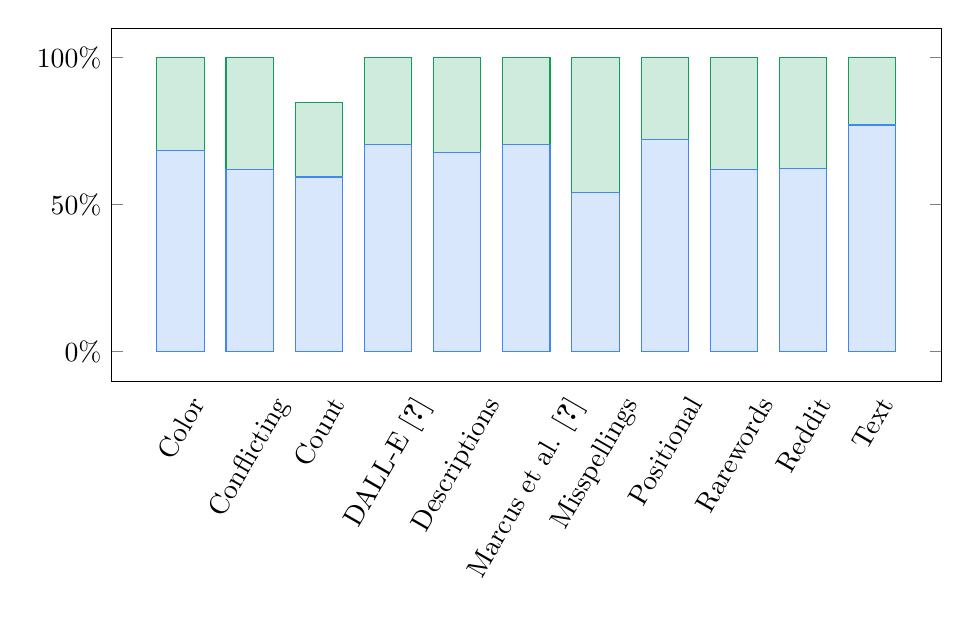
\begin{tikzpicture}

\definecolor{google_blue}{RGB}{66,133,244}
\definecolor{google_red}{RGB}{219,68,55}
\definecolor{google_yellow}{RGB}{194,144,0}
\definecolor{google_green}{RGB}{15,157,88}

\begin{axis}[
name=fidelity,
width=\textwidth,
height=0.5\textwidth,
ybar stacked,
ymin=-0.1,
ymax=1.1,
xtick=data,
xtick style={draw=none},
symbolic x coords={Color,Conflicting,Count,DALL-E \cite{ramesh-dalle},Descriptions,Marcus et al. \cite{marcus-arxiv-2022},Misspellings,Positional,Rarewords,Reddit,Text},
x tick label style={rotate=60},
ytick={0,0.5,1},
yticklabels={0\%, 50\%, 100\%},
legend style={font=\tiny},
legend cell align=left,
legend image code/.code={
    \draw [#1] (0cm, -0.1cm) rectangle (0.2cm, 0.25cm);
},
legend style={
draw=none,
at={(0.5, 1.1)},anchor=south,
legend columns=3,
/tikz/every even column/.append style={column sep=0.2cm}
},
bar width=0.6cm,
]

\addplot+[
    fill=google_blue,
    fill opacity=0.2,
    draw=google_blue
] coordinates {
(Color, 0.685)
(Conflicting, 0.619)
(Count, 0.594)
(DALL-E \cite{ramesh-dalle}, 0.704)
(Descriptions, 0.678)
(Marcus et al. \cite{marcus-arxiv-2022}, 0.705)
(Misspellings, 0.540)
(Positional, 0.721)
(Rarewords, 0.621)
(Reddit, 0.623)
(Text, 0.771)
};

\addplot+[
fill=google_green,
fill opacity=0.2,
draw=google_green
] coordinates {
(Color, 0.315)
(Conflicting, 0.381)
(Count, 0.252)
(DALL-E \cite{ramesh-dalle}, 0.296)
(Descriptions, 0.322)
(Marcus et al. \cite{marcus-arxiv-2022}, 0.295)
(Misspellings, 0.460)
(Positional, 0.279)
(Rarewords, 0.379)
(Reddit, 0.377)
(Text, 0.229)
};

\legend{}
\end{axis}

\end{tikzpicture}
    \caption{Fidelity}
    \label{fig:drawit_vs_dalle2_detailed_alignment_fidelity}
    \end{subfigure}
    \caption{\name vs DALL-E 2 on \benchmarkname \subref{fig:drawit_vs_dalle2_detailed_alignment_alignment}) image-text alignment, and \subref{fig:drawit_vs_dalle2_detailed_alignment_fidelity}) image fidelity.}
    \label{fig:drawit_vs_dalle2_detailed_alignment}
\end{figure}


\begin{figure}
    \centering
    \begin{subfigure}[t]{\textwidth}
    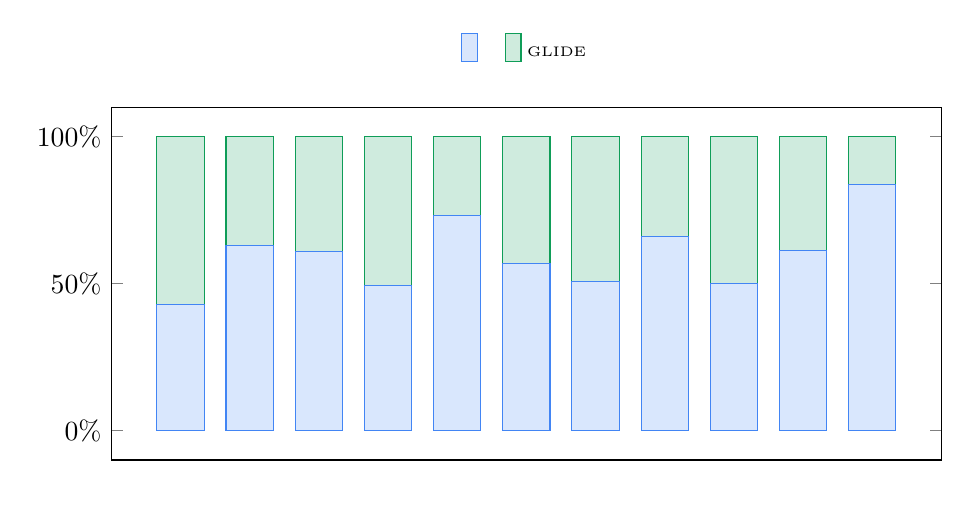
\begin{tikzpicture}

\definecolor{google_blue}{RGB}{66,133,244}
\definecolor{google_red}{RGB}{219,68,55}
\definecolor{google_yellow}{RGB}{194,144,0}
\definecolor{google_green}{RGB}{15,157,88}

\begin{axis}[
name=fidelity,
width=\textwidth,
height=0.5\textwidth,
ybar stacked,
ymin=-0.1,
ymax=1.1,
xtick=data,
xtick style={draw=none},
symbolic x coords={Colors,Conflicting,Counting,DALL-E \cite{ramesh-dalle},Descriptions,Marcus et al. \cite{marcus-arxiv-2022},Misspellings,Positional,Rare Words,Reddit,Text},
xticklabels={},
x tick label style={rotate=30},
ytick={0,0.5,1},
yticklabels={0\%, 50\%, 100\%},
legend style={font=\tiny},
legend cell align=left,
legend image code/.code={
    \draw [#1] (0cm, -0.1cm) rectangle (0.2cm, 0.25cm);
},
legend style={
draw=none,
at={(0.5, 1.1)},anchor=south,
legend columns=3,
/tikz/every even column/.append style={column sep=0.2cm}
},
bar width=0.6cm,
]

\addplot+[
    fill=google_blue,
    fill opacity=0.2,
    draw=google_blue
] coordinates {
(Colors, 0.429)
(Conflicting, 0.628)
(Counting, 0.609)
(DALL-E \cite{ramesh-dalle}, 0.493)
(Descriptions, 0.730)
(Marcus et al. \cite{marcus-arxiv-2022}, 0.568)
(Misspellings, 0.506)
(Positional, 0.659)
(Rare Words, 0.500)
(Reddit, 0.613)
(Text, 0.837)
};

\addplot+[
fill=google_green,
fill opacity=0.2,
draw=google_green
] coordinates {
(Colors, 0.571)
(Conflicting, 0.372)
(Counting, 0.391)
(DALL-E \cite{ramesh-dalle}, 0.507)
(Descriptions, 0.270)
(Marcus et al. \cite{marcus-arxiv-2022}, 0.432)
(Misspellings, 0.494)
(Positional, 0.341)
(Rare Words, 0.500)
(Reddit, 0.387)
(Text, 0.163)
};

\legend{\name, GLIDE}
\end{axis}

\end{tikzpicture}
    \caption{Alignment}
    \label{fig:drawit_vs_glide_detailed_alignment_alignment}
    \vspace*{0.5cm}
    \end{subfigure}
    \begin{subfigure}[t]{\textwidth}
    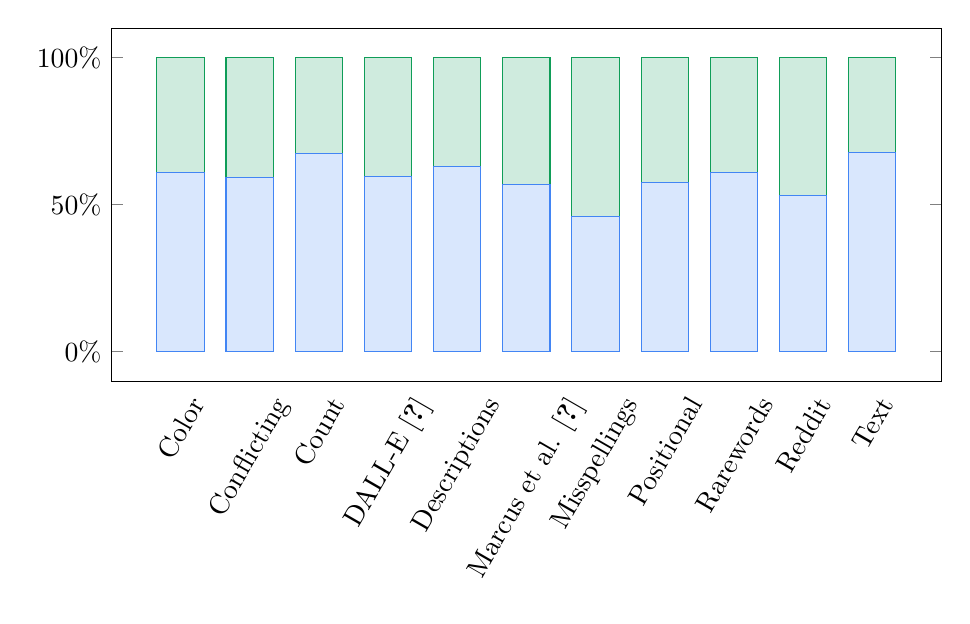
\begin{tikzpicture}

\definecolor{google_blue}{RGB}{66,133,244}
\definecolor{google_red}{RGB}{219,68,55}
\definecolor{google_yellow}{RGB}{194,144,0}
\definecolor{google_green}{RGB}{15,157,88}

\begin{axis}[
name=fidelity,
width=\textwidth,
height=0.5\textwidth,
ybar stacked,
ymin=-0.1,
ymax=1.1,
xtick=data,
xtick style={draw=none},
symbolic x coords={Color,Conflicting,Count,DALL-E \cite{ramesh-dalle},Descriptions,Marcus et al. \cite{marcus-arxiv-2022},Misspellings,Positional,Rarewords,Reddit,Text},
x tick label style={rotate=60},
ytick={0,0.5,1},
yticklabels={0\%, 50\%, 100\%},
legend style={font=\tiny},
legend cell align=left,
legend image code/.code={
    \draw [#1] (0cm, -0.1cm) rectangle (0.2cm, 0.25cm);
},
legend style={
draw=none,
at={(0.5, 1.1)},anchor=south,
legend columns=3,
/tikz/every even column/.append style={column sep=0.2cm}
},
bar width=0.6cm,
]

\addplot+[
    fill=google_blue,
    fill opacity=0.2,
    draw=google_blue
] coordinates {
(Color, 0.610)
(Conflicting, 0.593)
(Count, 0.674)
(DALL-E \cite{ramesh-dalle}, 0.597)
(Descriptions, 0.631)
(Marcus et al. \cite{marcus-arxiv-2022}, 0.568)
(Misspellings, 0.459)
(Positional, 0.575)
(Rarewords, 0.609)
(Reddit, 0.531)
(Text, 0.677)
};

\addplot+[
fill=google_green,
fill opacity=0.2,
draw=google_green
] coordinates {
(Color, 0.390)
(Conflicting, 0.407)
(Count, 0.326)
(DALL-E \cite{ramesh-dalle}, 0.403)
(Descriptions, 0.369)
(Marcus et al. \cite{marcus-arxiv-2022}, 0.432)
(Misspellings, 0.541)
(Positional, 0.425)
(Rarewords, 0.391)
(Reddit, 0.469)
(Text, 0.323)
};

\legend{}
\end{axis}

\end{tikzpicture}
    \caption{Fidelity}
    \label{fig:drawit_vs_glide_detailed_alignment_fidelity}
    \end{subfigure}
    \caption{\name vs GLIDE on \benchmarkname \subref{fig:drawit_vs_glide_detailed_alignment_alignment}) image-text alignment, and \subref{fig:drawit_vs_glide_detailed_alignment_fidelity}) image fidelity.}
    \label{fig:drawit_vs_glide_detailed_alignment}
\end{figure}

\begin{figure}[t]
\centering
\begin{tabular}{c@{\hskip 1pt}c@{\hskip 8pt}c@{\hskip 1pt}c}
\multicolumn{2}{c}{\name (Ours)} & \multicolumn{2}{c}{DALL-E 2 \cite{ramesh-dalle2}} \\
{\includegraphics[width=0.2\textwidth]{figures/drawit_vs_dalle2/cow_alien/drawit_1.jpeg}} &
{\includegraphics[width=0.2\textwidth]{figures/drawit_vs_dalle2/cow_alien/drawit_2.jpeg}} &
{\includegraphics[width=0.2\textwidth]{figures/drawit_vs_dalle2/cow_alien/dalle2_1.jpeg}} &
{\includegraphics[width=0.2\textwidth]{figures/drawit_vs_dalle2/cow_alien/dalle2_2.jpeg} }\\
{\includegraphics[width=0.2\textwidth]{figures/drawit_vs_dalle2/cow_alien/drawit_3.jpeg}} &
{\includegraphics[width=0.2\textwidth]{figures/drawit_vs_dalle2/cow_alien/drawit_4.jpeg}} &
{\includegraphics[width=0.2\textwidth]{figures/drawit_vs_dalle2/cow_alien/dalle2_3.jpeg}} &
{\includegraphics[width=0.2\textwidth]{figures/drawit_vs_dalle2/cow_alien/dalle2_4.jpeg}}\\
\multicolumn{4}{c}{Hovering cow abducting aliens.} \\
\multicolumn{4}{c}{} \\
{\includegraphics[width=0.2\textwidth]{figures/drawit_vs_dalle2/greek_statue/drawit_1.jpeg}} &
{\includegraphics[width=0.2\textwidth]{figures/drawit_vs_dalle2/greek_statue/drawit_2.jpeg}} &
{\includegraphics[width=0.2\textwidth]{figures/drawit_vs_dalle2/greek_statue/dalle2_1.jpeg}} &
{\includegraphics[width=0.2\textwidth]{figures/drawit_vs_dalle2/greek_statue/dalle2_2.jpeg} }\\
{\includegraphics[width=0.2\textwidth]{figures/drawit_vs_dalle2/greek_statue/drawit_3.jpeg}} &
{\includegraphics[width=0.2\textwidth]{figures/drawit_vs_dalle2/greek_statue/drawit_4.jpeg}} &
{\includegraphics[width=0.2\textwidth]{figures/drawit_vs_dalle2/greek_statue/dalle2_3.jpeg}} &
{\includegraphics[width=0.2\textwidth]{figures/drawit_vs_dalle2/greek_statue/dalle2_4.jpeg}}\\
\multicolumn{4}{c}{Greek statue of a man tripping over a cat.}
\end{tabular}

\caption{Example qualitative comparisons between \name and DALL-E 2 \cite{ramesh-dalle2} on \benchmarkname prompts from Reddit category.}
\label{fig:drawit_vs_dalle2_reddit}
\end{figure}

\begin{figure}[t]
\centering
\begin{tabular}{c@{\hskip 1pt}c@{\hskip 8pt}c@{\hskip 1pt}c}
\multicolumn{2}{c}{\name (Ours)} & \multicolumn{2}{c}{DALL-E 2 \cite{ramesh-dalle2}} \\
{\includegraphics[width=0.2\textwidth]{figures/drawit_vs_dalle2/yellowbook_redvase/drawit_1.jpeg}} &
{\includegraphics[width=0.2\textwidth]{figures/drawit_vs_dalle2/yellowbook_redvase/drawit_2.jpeg}} &
{\includegraphics[width=0.2\textwidth]{figures/drawit_vs_dalle2/yellowbook_redvase/dalle2_1.jpeg}} &
{\includegraphics[width=0.2\textwidth]{figures/drawit_vs_dalle2/yellowbook_redvase/dalle2_2.jpeg} }\\
{\includegraphics[width=0.2\textwidth]{figures/drawit_vs_dalle2/yellowbook_redvase/drawit_3.jpeg}} &
{\includegraphics[width=0.2\textwidth]{figures/drawit_vs_dalle2/yellowbook_redvase/drawit_4.jpeg}} &
{\includegraphics[width=0.2\textwidth]{figures/drawit_vs_dalle2/yellowbook_redvase/dalle2_3.jpeg}} &
{\includegraphics[width=0.2\textwidth]{figures/drawit_vs_dalle2/yellowbook_redvase/dalle2_4.jpeg}}\\
\multicolumn{4}{c}{A yellow book and a red vase.} \\
\multicolumn{4}{c}{} \\
{\includegraphics[width=0.2\textwidth]{figures/drawit_vs_dalle2/blackapple_greenbag/drawit_1.jpeg}} &
{\includegraphics[width=0.2\textwidth]{figures/drawit_vs_dalle2/blackapple_greenbag/drawit_2.jpeg}} &
{\includegraphics[width=0.2\textwidth]{figures/drawit_vs_dalle2/blackapple_greenbag/dalle2_1.jpeg}} &
{\includegraphics[width=0.2\textwidth]{figures/drawit_vs_dalle2/blackapple_greenbag/dalle2_2.jpeg} }\\
{\includegraphics[width=0.2\textwidth]{figures/drawit_vs_dalle2/blackapple_greenbag/drawit_3.jpeg}} &
{\includegraphics[width=0.2\textwidth]{figures/drawit_vs_dalle2/blackapple_greenbag/drawit_4.jpeg}} &
{\includegraphics[width=0.2\textwidth]{figures/drawit_vs_dalle2/blackapple_greenbag/dalle2_3.jpeg}} &
{\includegraphics[width=0.2\textwidth]{figures/drawit_vs_dalle2/blackapple_greenbag/dalle2_4.jpeg}}\\
\multicolumn{4}{c}{A black apple and a green backpack.}
\end{tabular}

\caption{Example qualitative comparisons between \name and DALL-E 2 \cite{ramesh-dalle2} on \benchmarkname prompts from Colors category. We observe that DALL-E 2 generally struggles with correctly assigning the colors to the objects especially for prompts with more than one object.}
\label{fig:drawit_vs_dalle2_colors}
\end{figure}

\begin{figure}[t]
\centering
\begin{tabular}{c@{\hskip 1pt}c@{\hskip 8pt}c@{\hskip 1pt}c}
\multicolumn{2}{c}{\name (Ours)} & \multicolumn{2}{c}{DALL-E 2 \cite{ramesh-dalle2}} \\
{\includegraphics[width=0.2\textwidth]{figures/drawit_vs_dalle2/horse_riding_astronaut/drawit_1.jpeg}} &
{\includegraphics[width=0.2\textwidth]{figures/drawit_vs_dalle2/horse_riding_astronaut/drawit_2.jpeg}} &
{\includegraphics[width=0.2\textwidth]{figures/drawit_vs_dalle2/horse_riding_astronaut/dalle2_1.jpeg}} &
{\includegraphics[width=0.2\textwidth]{figures/drawit_vs_dalle2/horse_riding_astronaut/dalle2_2.jpeg} }\\
{\includegraphics[width=0.2\textwidth]{figures/drawit_vs_dalle2/horse_riding_astronaut/drawit_3.jpeg}} &
{\includegraphics[width=0.2\textwidth]{figures/drawit_vs_dalle2/horse_riding_astronaut/drawit_4.jpeg}} &
{\includegraphics[width=0.2\textwidth]{figures/drawit_vs_dalle2/horse_riding_astronaut/dalle2_3.jpeg}} &
{\includegraphics[width=0.2\textwidth]{figures/drawit_vs_dalle2/horse_riding_astronaut/dalle2_4.jpeg}}\\
\multicolumn{4}{c}{A horse riding an astronaut.} \\
\multicolumn{4}{c}{} \\
{\includegraphics[width=0.2\textwidth]{figures/drawit_vs_dalle2/panda_latte_art/drawit_1.jpeg}} &
{\includegraphics[width=0.2\textwidth]{figures/drawit_vs_dalle2/panda_latte_art/drawit_2.jpeg}} &
{\includegraphics[width=0.2\textwidth]{figures/drawit_vs_dalle2/panda_latte_art/dalle2_1.jpeg}} &
{\includegraphics[width=0.2\textwidth]{figures/drawit_vs_dalle2/panda_latte_art/dalle2_2.jpeg} }\\
{\includegraphics[width=0.2\textwidth]{figures/drawit_vs_dalle2/panda_latte_art/drawit_3.jpeg}} &
{\includegraphics[width=0.2\textwidth]{figures/drawit_vs_dalle2/panda_latte_art/drawit_4.jpeg}} &
{\includegraphics[width=0.2\textwidth]{figures/drawit_vs_dalle2/panda_latte_art/dalle2_3.jpeg}} &
{\includegraphics[width=0.2\textwidth]{figures/drawit_vs_dalle2/panda_latte_art/dalle2_4.jpeg}}\\
\multicolumn{4}{c}{A panda making latte art.}
\end{tabular}

\caption{Example qualitative comparisons between \name and DALL-E 2 \cite{ramesh-dalle2} on \benchmarkname prompts from Conflicting category. We observe that both DALL-E 2 and \name struggle generating well aligned images for this category. However, \name often generates some well aligned samples, e.g. ``A panda making latte art.''.}
\label{fig:drawit_vs_dalle2_conflicting}
\end{figure}

\begin{figure}[t]
\centering
\begin{tabular}{c@{\hskip 1pt}c@{\hskip 8pt}c@{\hskip 1pt}c}
\multicolumn{2}{c}{\name (Ours)} & \multicolumn{2}{c}{DALL-E 2 \cite{ramesh-dalle2}} \\
{\includegraphics[width=0.2\textwidth]{figures/drawit_vs_dalle2/glasses_on_table/drawit_1.jpeg}} &
{\includegraphics[width=0.2\textwidth]{figures/drawit_vs_dalle2/glasses_on_table/drawit_2.jpeg}} &
{\includegraphics[width=0.2\textwidth]{figures/drawit_vs_dalle2/glasses_on_table/dalle2_1.jpeg}} &
{\includegraphics[width=0.2\textwidth]{figures/drawit_vs_dalle2/glasses_on_table/dalle2_2.jpeg} }\\
{\includegraphics[width=0.2\textwidth]{figures/drawit_vs_dalle2/glasses_on_table/drawit_3.jpeg}} &
{\includegraphics[width=0.2\textwidth]{figures/drawit_vs_dalle2/glasses_on_table/drawit_4.jpeg}} &
{\includegraphics[width=0.2\textwidth]{figures/drawit_vs_dalle2/glasses_on_table/dalle2_3.jpeg}} &
{\includegraphics[width=0.2\textwidth]{figures/drawit_vs_dalle2/glasses_on_table/dalle2_4.jpeg}}\\
\multicolumn{4}{c}{A couple of glasses are sitting on a table.} \\
\multicolumn{4}{c}{} \\
{\includegraphics[width=0.2\textwidth]{figures/drawit_vs_dalle2/cube_brick/drawit_1.jpeg}} &
{\includegraphics[width=0.2\textwidth]{figures/drawit_vs_dalle2/cube_brick/drawit_2.jpeg}} &
{\includegraphics[width=0.2\textwidth]{figures/drawit_vs_dalle2/cube_brick/dalle2_1.jpeg}} &
{\includegraphics[width=0.2\textwidth]{figures/drawit_vs_dalle2/cube_brick/dalle2_2.jpeg} }\\
{\includegraphics[width=0.2\textwidth]{figures/drawit_vs_dalle2/cube_brick/drawit_3.jpeg}} &
{\includegraphics[width=0.2\textwidth]{figures/drawit_vs_dalle2/cube_brick/drawit_4.jpeg}} &
{\includegraphics[width=0.2\textwidth]{figures/drawit_vs_dalle2/cube_brick/dalle2_3.jpeg}} &
{\includegraphics[width=0.2\textwidth]{figures/drawit_vs_dalle2/cube_brick/dalle2_4.jpeg}}\\
\multicolumn{4}{c}{A cube made of brick. A cube with the texture of brick.}
\end{tabular}

\caption{Example qualitative comparisons between \name and DALL-E 2 \cite{ramesh-dalle2} on \benchmarkname prompts from DALL-E category.}
\label{fig:drawit_vs_dalle2_dalle}
\end{figure}

\begin{figure}[t]
\centering
\begin{tabular}{c@{\hskip 1pt}c@{\hskip 8pt}c@{\hskip 1pt}c}
\multicolumn{2}{c}{\name (Ours)} & \multicolumn{2}{c}{DALL-E 2 \cite{ramesh-dalle2}} \\
{\includegraphics[width=0.2\textwidth]{figures/drawit_vs_dalle2/hello_world/drawit_1.jpeg}} &
{\includegraphics[width=0.2\textwidth]{figures/drawit_vs_dalle2/hello_world/drawit_2.jpeg}} &
{\includegraphics[width=0.2\textwidth]{figures/drawit_vs_dalle2/hello_world/dalle2_1.jpeg}} &
{\includegraphics[width=0.2\textwidth]{figures/drawit_vs_dalle2/hello_world/dalle2_2.jpeg} }\\
{\includegraphics[width=0.2\textwidth]{figures/drawit_vs_dalle2/hello_world/drawit_3.jpeg}} &
{\includegraphics[width=0.2\textwidth]{figures/drawit_vs_dalle2/hello_world/drawit_4.jpeg}} &
{\includegraphics[width=0.2\textwidth]{figures/drawit_vs_dalle2/hello_world/dalle2_3.jpeg}} &
{\includegraphics[width=0.2\textwidth]{figures/drawit_vs_dalle2/hello_world/dalle2_4.jpeg}}\\
\multicolumn{4}{c}{New York Skyline with Hello World written with fireworks on the sky.} \\
\multicolumn{4}{c}{} \\
{\includegraphics[width=0.2\textwidth]{figures/drawit_vs_dalle2/text_to_image/drawit_1.jpeg}} &
{\includegraphics[width=0.2\textwidth]{figures/drawit_vs_dalle2/text_to_image/drawit_2.jpeg}} &
{\includegraphics[width=0.2\textwidth]{figures/drawit_vs_dalle2/text_to_image/dalle2_1.jpeg}} &
{\includegraphics[width=0.2\textwidth]{figures/drawit_vs_dalle2/text_to_image/dalle2_2.jpeg} }\\
{\includegraphics[width=0.2\textwidth]{figures/drawit_vs_dalle2/text_to_image/drawit_3.jpeg}} &
{\includegraphics[width=0.2\textwidth]{figures/drawit_vs_dalle2/text_to_image/drawit_4.jpeg}} &
{\includegraphics[width=0.2\textwidth]{figures/drawit_vs_dalle2/text_to_image/dalle2_3.jpeg}} &
{\includegraphics[width=0.2\textwidth]{figures/drawit_vs_dalle2/text_to_image/dalle2_4.jpeg}}\\
\multicolumn{4}{c}{A storefront with Text to Image written on it.}
\end{tabular}

\caption{Example qualitative comparisons between \name and DALL-E 2 \cite{ramesh-dalle2} on \benchmarkname prompts from Text category. \name is significantly better than DALL-E 2 in prompts with quoted text.}
\label{fig:drawit_vs_dalle2_text}
\end{figure}



\FloatBarrier
\begin{figure}[htb]
\centering
\begin{tabular}{c@{\hskip 1pt}c@{\hskip 8pt}c@{\hskip 1pt}c}
\multicolumn{2}{c}{\name (Ours)} & \multicolumn{2}{c}{GLIDE \cite{nichol-glide}} \\
{\includegraphics[width=0.2\textwidth]{figures/drawit_vs_dalle2/cow_alien/drawit_1.jpeg}} &
{\includegraphics[width=0.2\textwidth]{figures/drawit_vs_dalle2/cow_alien/drawit_2.jpeg}} &
{\includegraphics[width=0.2\textwidth]{figures/glide/029_00.jpg}} &
{\includegraphics[width=0.2\textwidth]{figures/glide/029_01.jpg}} \\
{\includegraphics[width=0.2\textwidth]{figures/drawit_vs_dalle2/cow_alien/drawit_3.jpeg}} &
{\includegraphics[width=0.2\textwidth]{figures/drawit_vs_dalle2/cow_alien/drawit_4.jpeg}} &
{\includegraphics[width=0.2\textwidth]{figures/glide/029_02.jpg}} &
{\includegraphics[width=0.2\textwidth]{figures/glide/029_03.jpg}} \\
\multicolumn{4}{c}{Hovering cow abducting aliens.} \\
\multicolumn{4}{c}{} \\
{\includegraphics[width=0.2\textwidth]{figures/drawit_vs_dalle2/greek_statue/drawit_1.jpeg}} &
{\includegraphics[width=0.2\textwidth]{figures/drawit_vs_dalle2/greek_statue/drawit_2.jpeg}} &
{\includegraphics[width=0.2\textwidth]{figures/glide/156_00.jpg}} &
{\includegraphics[width=0.2\textwidth]{figures/glide/156_01.jpg}} \\
{\includegraphics[width=0.2\textwidth]{figures/drawit_vs_dalle2/greek_statue/drawit_3.jpeg}} &
{\includegraphics[width=0.2\textwidth]{figures/drawit_vs_dalle2/greek_statue/drawit_4.jpeg}} &
{\includegraphics[width=0.2\textwidth]{figures/glide/156_02.jpg}} &
{\includegraphics[width=0.2\textwidth]{figures/glide/156_03.jpg}} \\
\multicolumn{4}{c}{Greek statue of a man tripping over a cat.}
\end{tabular}
\caption{Example qualitative comparisons between \name and GLIDE \cite{nichol-glide} on \benchmarkname prompts from Reddit category.}
\label{fig:drawit_vs_glide_reddit}
\end{figure}

\begin{figure}[t]
\centering
\begin{tabular}{c@{\hskip 1pt}c@{\hskip 8pt}c@{\hskip 1pt}c}
\multicolumn{2}{c}{\name (Ours)} & \multicolumn{2}{c}{GLIDE \cite{nichol-glide}} \\
{\includegraphics[width=0.2\textwidth]{figures/drawit_vs_dalle2/yellowbook_redvase/drawit_1.jpeg}} &
{\includegraphics[width=0.2\textwidth]{figures/drawit_vs_dalle2/yellowbook_redvase/drawit_2.jpeg}} &
{\includegraphics[width=0.2\textwidth]{figures/glide/019_00.jpg}} &
{\includegraphics[width=0.2\textwidth]{figures/glide/019_01.jpg}} \\
{\includegraphics[width=0.2\textwidth]{figures/drawit_vs_dalle2/yellowbook_redvase/drawit_3.jpeg}} &
{\includegraphics[width=0.2\textwidth]{figures/drawit_vs_dalle2/yellowbook_redvase/drawit_4.jpeg}} &
{\includegraphics[width=0.2\textwidth]{figures/glide/019_02.jpg}} &
{\includegraphics[width=0.2\textwidth]{figures/glide/019_03.jpg}} \\
\multicolumn{4}{c}{A yellow book and a red vase.} \\
\multicolumn{4}{c}{} \\
{\includegraphics[width=0.2\textwidth]{figures/drawit_vs_dalle2/blackapple_greenbag/drawit_1.jpeg}} &
{\includegraphics[width=0.2\textwidth]{figures/drawit_vs_dalle2/blackapple_greenbag/drawit_2.jpeg}} &
{\includegraphics[width=0.2\textwidth]{figures/glide/022_00.jpg}} &
{\includegraphics[width=0.2\textwidth]{figures/glide/022_01.jpg}} \\
{\includegraphics[width=0.2\textwidth]{figures/drawit_vs_dalle2/blackapple_greenbag/drawit_3.jpeg}} &
{\includegraphics[width=0.2\textwidth]{figures/drawit_vs_dalle2/blackapple_greenbag/drawit_4.jpeg}} &
{\includegraphics[width=0.2\textwidth]{figures/glide/022_02.jpg}} &
{\includegraphics[width=0.2\textwidth]{figures/glide/022_03.jpg}} \\
\multicolumn{4}{c}{A black apple and a green backpack.}
\end{tabular}

\caption{Example qualitative comparisons between \name and GLIDE \cite{nichol-glide} on \benchmarkname prompts from Colors category. We observe that GLIDE is better than DALL-E 2 in assigning the colors to the objects.}
\label{fig:drawit_vs_glide_colors}
\end{figure}

\begin{figure}[t]
\centering
\begin{tabular}{c@{\hskip 1pt}c@{\hskip 8pt}c@{\hskip 1pt}c}
\multicolumn{2}{c}{\name (Ours)} & \multicolumn{2}{c}{GLIDE \cite{nichol-glide}} \\
{\includegraphics[width=0.2\textwidth]{figures/drawit_vs_dalle2/horse_riding_astronaut/drawit_1.jpeg}} &
{\includegraphics[width=0.2\textwidth]{figures/drawit_vs_dalle2/horse_riding_astronaut/drawit_2.jpeg}} &
{\includegraphics[width=0.2\textwidth]{figures/glide/025_00.jpg}} &
{\includegraphics[width=0.2\textwidth]{figures/glide/025_01.jpg}} \\
{\includegraphics[width=0.2\textwidth]{figures/drawit_vs_dalle2/horse_riding_astronaut/drawit_3.jpeg}} &
{\includegraphics[width=0.2\textwidth]{figures/drawit_vs_dalle2/horse_riding_astronaut/drawit_4.jpeg}} &
{\includegraphics[width=0.2\textwidth]{figures/glide/025_02.jpg}} &
{\includegraphics[width=0.2\textwidth]{figures/glide/025_03.jpg}} \\
\multicolumn{4}{c}{A horse riding an astronaut.} \\
\multicolumn{4}{c}{} \\
{\includegraphics[width=0.2\textwidth]{figures/drawit_vs_dalle2/panda_latte_art/drawit_1.jpeg}} &
{\includegraphics[width=0.2\textwidth]{figures/drawit_vs_dalle2/panda_latte_art/drawit_2.jpeg}} &
{\includegraphics[width=0.2\textwidth]{figures/glide/030_00.jpg}} &
{\includegraphics[width=0.2\textwidth]{figures/glide/030_01.jpg}} \\
{\includegraphics[width=0.2\textwidth]{figures/drawit_vs_dalle2/panda_latte_art/drawit_3.jpeg}} &
{\includegraphics[width=0.2\textwidth]{figures/drawit_vs_dalle2/panda_latte_art/drawit_4.jpeg}} &
{\includegraphics[width=0.2\textwidth]{figures/glide/030_02.jpg}} &
{\includegraphics[width=0.2\textwidth]{figures/glide/030_03.jpg}} \\
\multicolumn{4}{c}{A panda making latte art.}
\end{tabular}

\caption{Example qualitative comparisons between \name and GLIDE \cite{nichol-glide} on \benchmarkname prompts from Conflicting category.}
\label{fig:drawit_vs_glide_conflicting}
\end{figure}

\begin{figure}[t]
\centering
\begin{tabular}{c@{\hskip 1pt}c@{\hskip 8pt}c@{\hskip 1pt}c}
\multicolumn{2}{c}{\name (Ours)} & \multicolumn{2}{c}{GLIDE \cite{nichol-glide}} \\
{\includegraphics[width=0.2\textwidth]{figures/drawit_vs_dalle2/glasses_on_table/drawit_1.jpeg}} &
{\includegraphics[width=0.2\textwidth]{figures/drawit_vs_dalle2/glasses_on_table/drawit_2.jpeg}} &
{\includegraphics[width=0.2\textwidth]{figures/glide/062_00.jpg}} &
{\includegraphics[width=0.2\textwidth]{figures/glide/062_01.jpg}} \\
{\includegraphics[width=0.2\textwidth]{figures/drawit_vs_dalle2/glasses_on_table/drawit_3.jpeg}} &
{\includegraphics[width=0.2\textwidth]{figures/drawit_vs_dalle2/glasses_on_table/drawit_4.jpeg}} &
{\includegraphics[width=0.2\textwidth]{figures/glide/062_02.jpg}} &
{\includegraphics[width=0.2\textwidth]{figures/glide/062_03.jpg}} \\
\multicolumn{4}{c}{A couple of glasses are sitting on a table.} \\
\multicolumn{4}{c}{} \\
{\includegraphics[width=0.2\textwidth]{figures/drawit_vs_dalle2/cube_brick/drawit_1.jpeg}} &
{\includegraphics[width=0.2\textwidth]{figures/drawit_vs_dalle2/cube_brick/drawit_2.jpeg}} &
{\includegraphics[width=0.2\textwidth]{figures/glide/059_00.jpg}} &
{\includegraphics[width=0.2\textwidth]{figures/glide/059_01.jpg}} \\
{\includegraphics[width=0.2\textwidth]{figures/drawit_vs_dalle2/cube_brick/drawit_3.jpeg}} &
{\includegraphics[width=0.2\textwidth]{figures/drawit_vs_dalle2/cube_brick/drawit_4.jpeg}} &
{\includegraphics[width=0.2\textwidth]{figures/glide/059_02.jpg}} &
{\includegraphics[width=0.2\textwidth]{figures/glide/059_03.jpg}} \\
\\
\multicolumn{4}{c}{A cube made of brick. A cube with the texture of brick.}
\end{tabular}

\caption{Example qualitative comparisons between \name and GLIDE \cite{nichol-glide} on \benchmarkname prompts from DALL-E category.}
\label{fig:drawit_vs_glide_dalle}
\end{figure}

\begin{figure}[t]
\centering
\begin{tabular}{c@{\hskip 1pt}c@{\hskip 8pt}c@{\hskip 1pt}c}
\multicolumn{2}{c}{\name (Ours)} & \multicolumn{2}{c}{GLIDE \cite{nichol-glide}} \\
{\includegraphics[width=0.2\textwidth]{figures/drawit_vs_dalle2/hello_world/drawit_1.jpeg}} &
{\includegraphics[width=0.2\textwidth]{figures/drawit_vs_dalle2/hello_world/drawit_2.jpeg}} &
{\includegraphics[width=0.2\textwidth]{figures/glide/193_00.jpg}} &
{\includegraphics[width=0.2\textwidth]{figures/glide/193_01.jpg}} \\
{\includegraphics[width=0.2\textwidth]{figures/drawit_vs_dalle2/hello_world/drawit_3.jpeg}} &
{\includegraphics[width=0.2\textwidth]{figures/drawit_vs_dalle2/hello_world/drawit_4.jpeg}} &
{\includegraphics[width=0.2\textwidth]{figures/glide/193_02.jpg}} &
{\includegraphics[width=0.2\textwidth]{figures/glide/193_03.jpg}} \\
\multicolumn{4}{c}{New York Skyline with Hello World written with fireworks on the sky.} \\
\multicolumn{4}{c}{} \\
{\includegraphics[width=0.2\textwidth]{figures/drawit_vs_dalle2/text_to_image/drawit_1.jpeg}} &
{\includegraphics[width=0.2\textwidth]{figures/drawit_vs_dalle2/text_to_image/drawit_2.jpeg}} &
{\includegraphics[width=0.2\textwidth]{figures/glide/181_00.jpg}} &
{\includegraphics[width=0.2\textwidth]{figures/glide/181_01.jpg}} \\
{\includegraphics[width=0.2\textwidth]{figures/drawit_vs_dalle2/text_to_image/drawit_3.jpeg}} &
{\includegraphics[width=0.2\textwidth]{figures/drawit_vs_dalle2/text_to_image/drawit_4.jpeg}} &
{\includegraphics[width=0.2\textwidth]{figures/glide/181_02.jpg}} &
{\includegraphics[width=0.2\textwidth]{figures/glide/181_03.jpg}} \\
\multicolumn{4}{c}{A storefront with Text to Image written on it.}
\end{tabular}

\caption{Example qualitative comparisons between \name and GLIDE \cite{nichol-glide} on \benchmarkname prompts from Text category. \name is significantly better than GLIDE too in prompts with quoted text.}
\label{fig:drawit_vs_glide_text}
\end{figure}



